% this file is called up by thesis.tex
% content in this file will be fed into the main document

\chapter{Replacement for Hit Correlation Step} % top level followed by
% section, subsection
\label{cha:mlp}

% ----------------------- contents from here ------------------------
% 
This chapter presents the replacement created using a Multi Layered
Perceptron (MLP) for the \textit{Hit Correlation Step} of the Karas
pipeline (see \ref{cha:karas-pipeline}). It is observed that a MLP is
able to identify causally related hits with a higher accuracy,
precision and recall compared to the PMC. The chapter begins by
explaining how the data is created followed by its visual examination.
The training and testing procedure for the model is explained next.
The chapter concludes with discussions of the experiment results and
next steps.

\section{Data Preparation}
\label{sec:mlp-data-prep}

A random sample was taken from the top 5 timeslices with the most
number of event hits for the creation of the MLP dataset, since these
timeslices contain the highest number of event hits compared to other
timeslices. This is useful since the main dataset is highly skewed and
using a timeslice with lesser number of event hits will proliferate
the skewed nature of the data in the MLP dataset once created. The
model is required to classify related and unrelated hits which can be
done by observing the space and time difference between the given
points. Since this phenomenon is consistent across the entire dataset,
training using a sample does not introduce any bias into the model.

% TODO find the mathematical term for the series, could be n^{2}-n!
Figure \ref{fig:mlp-data} summarizes the MLP dataset creation
process. With an input data of shape $(n, 4)$ (\emph{n} rows
and 4 columns representing \emph{x, y, z, and t}), an output
data of shape \texttt{($\sum_{k=n-1}^{1}k$, 9)} is obtained. A
significant rise in the number of rows is observed since each row
(representing a single hit) is paired with the remaining unique rows.
The output dataset consists of 9 columns due to the presence of
\emph{x, y, z and t} columns of two hits plus the label column.

\begin{figure}[t]
  \centering
  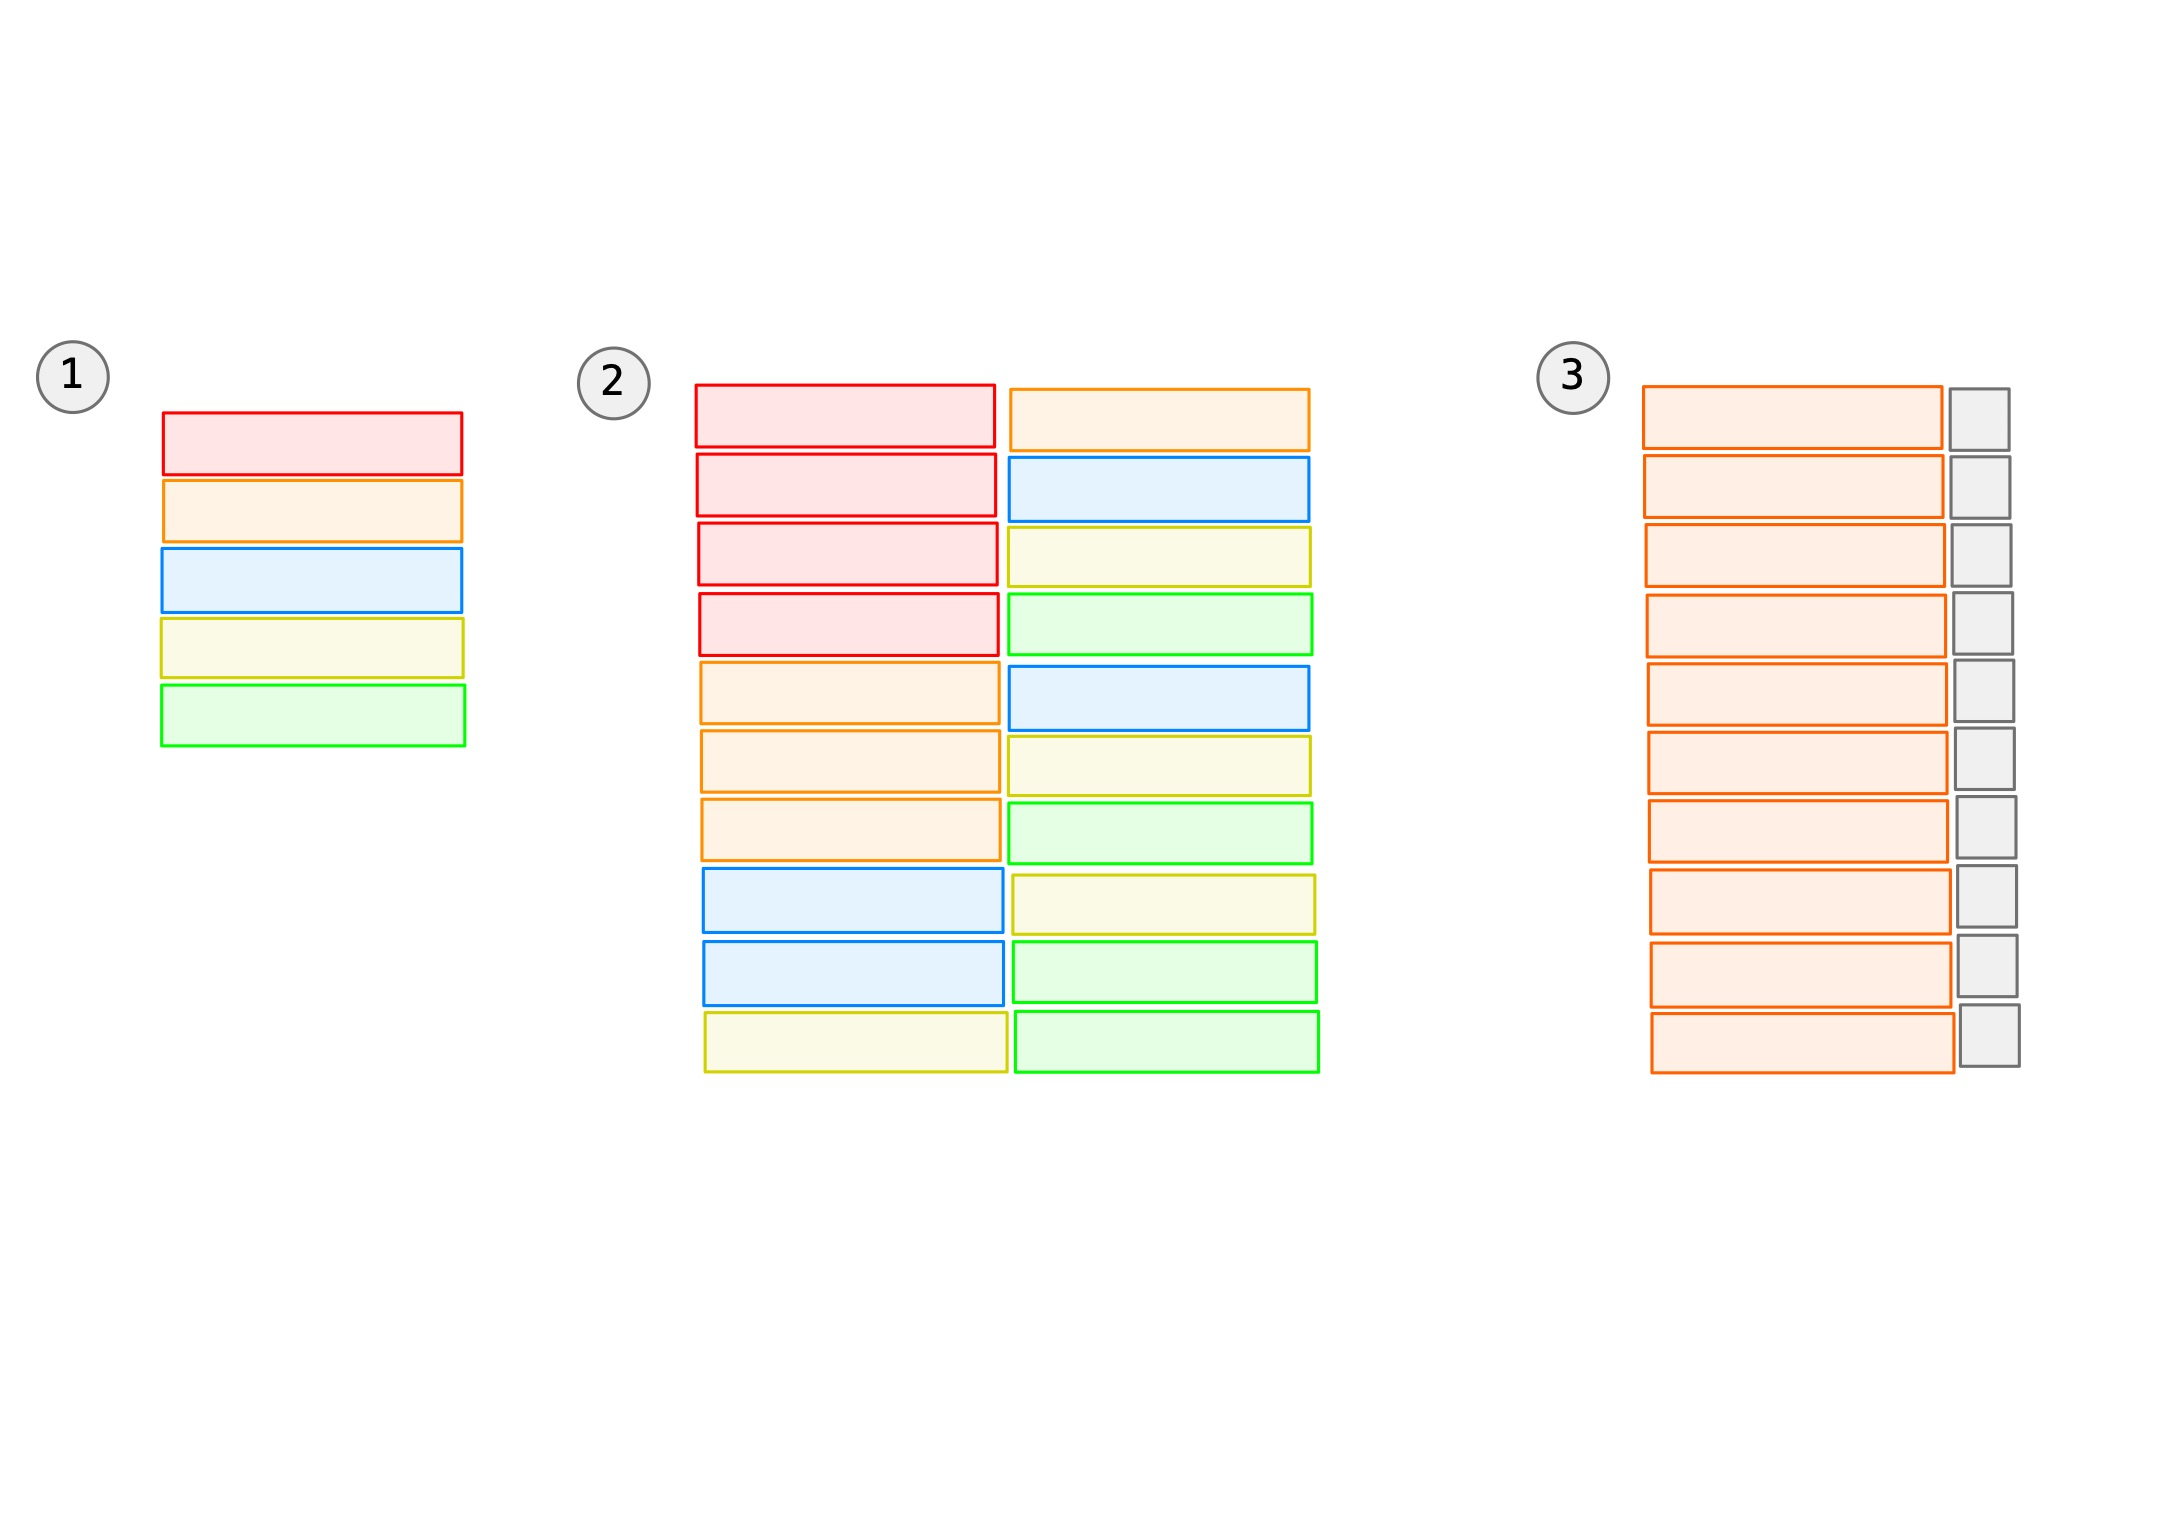
\includegraphics[width=\textwidth]{mlp-data.jpg}
  \caption{Overview of MLP dataset creation procedure. \textbf{(1)}
    The main dataset where each row represents a hit, here an example
    set containing 5 rows is shown for simplicity. \textbf{(2)} The
    MLP dataset is generated from the main dataset consisting of all
    unique pairs of hits. Algorithmically, this is done by pairing
    each hit with the subsequent hits below it as demonstrated with
    the use of colors. \textbf{(3)} The difference between the hits is
    taken (dark orange) and a label is assigned to each row (gray).}
  \label{fig:mlp-data}
\end{figure}

The label column is populated based on the values of the
\texttt{event\_id} column of the two hits. The row is assigned a label
of 1 if the two hits have the same event id, which signifies that they
originated from the same neutrino event and hence are causally related
to each other. If the event id of the two hits are not the same then
they are assigned a label of 0.

Better model performance was observed when the model was trained with
the difference between hits in time and space. As a result, the
pattern matrix was modified such that a dataset of shape
\texttt{$\sum_{k=n-1}^{1}k$, 5} was obtained. The fist 4 column being the
difference of the \emph{x, y, z and t} columns and the last column
being the label.

\subsection{Preparation of Training Data}
\label{sec:mlp-data-prep-train}

The main dataset is highly skewed, with the \textbf{majority class}
being hits from background noise and the \textbf{minority class} being
hits from neutrino events. Thus, the \textit{pattern matrix} dataset
is also skewed with the minority class being related hits and majority
class being unrelated hits. In binary classification, the majority
class is also referred to as the \textbf{negative class} (since it
usually has a label of 0) and the minority class is referred to as the
\textbf{positive class} (since usually has a label of 1). Henceforth
this alternative naming convention is used in this report.

Training the model with such a skewed dataset will result in a model
that is biased to the majority class. To combat this problem, the
majority class is undersampled \cite{CITEME} such that the number of
examples for each class is the same. Figure \ref{fig:mlp-train-dist}
shows the distribution of a random sample of the MLP training set. It
is observed that the related hits occur close to one another in space
 and time whilst the noise hits are scattered throughout.

 \begin{figure}[h]
   \centering
   \caption{Distribution of MLP training dataset.}
   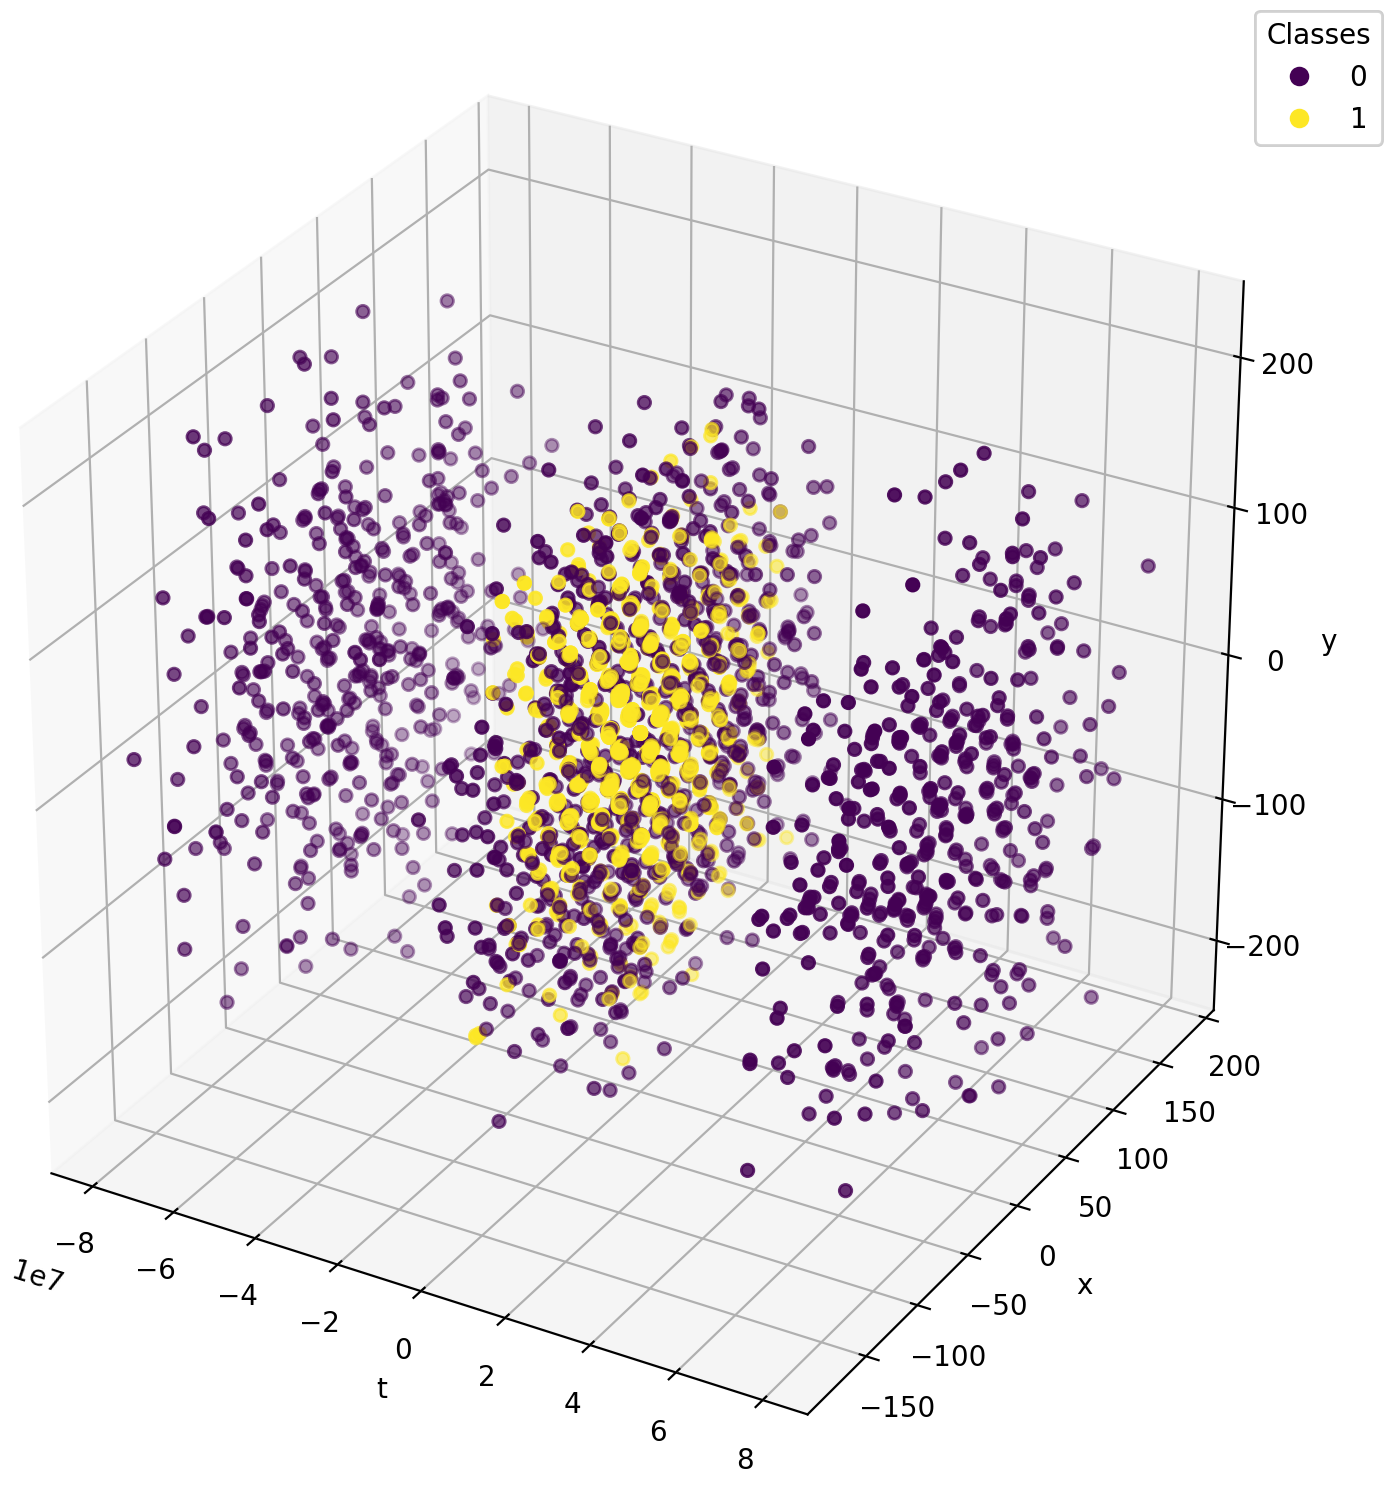
\includegraphics[width=\textwidth]{mlp-train-dist.png}
   \label{fig:mlp-train-dist}
 \end{figure}

\subsection{Preparation of Testing Data}
\label{sec:mlp-data-prep-test}

Whilst the training dataset contains equal number of examples for each
class, the testing dataset maintains it's skewed distribution since
this represents realistic data which the model will be required to
classify. Four variants of the testing dataset with varying level of
examples of related hits were created as listed below. In practise,
the pipeline will observe timeslices which contain no to very few
related hits, thus the performance of the model on test set 1 and 2
are of vital importance.

\begin{enumerate}
\item[\textbf{TS1}.] No related hits
\item[\textbf{TS2}.] Less than 25 related hits
\item[\textbf{TS3}.] Less than 500 related hits
\item[\textbf{TS4}.] Less than 1500 related hits
\end{enumerate}

\section{Model Description}
\label{sec:mlp-model-desc}

The expectation of the model is to identify if two given points are
causally related to each other or not. As revealed through data
exploration in Chapter \ref{cha:data-exploration}, hits originating from
neutrino events occur close to each other in space and time. Thus, The
expectation from the model is to learn this phenomenon by training
over pairs of points and classify unseen data as related or unrelated.

\begin{table}[t]
  \centering
  \begin{tabular}{rr}
    \hline
    Loss & BCELoss \\
    Optimizer & Stocastic Gradient Descent with learning rate of $0.001$ \\
    Hidden activation function & ReLu \\
    Output activation function & Sigmoid \\
    Training batch size & 4 \\
    Testing batch size & 16 \\
    \hline
  \end{tabular}
  \caption{GCN Model Parameter Summary.}
  \label{tab:gcn-model-param}
\end{table}

% TODO rational for small training batch size and large testing batch
% size
The parameters of the model are summarized in Table
\ref{tab:mlp-model-param}. Being a binary classification task, the
\textit{Binary Cross Entropy Loss (BCELoss)} was selected as the loss
function since it has been established as the standard loss function
for binary classification tasks \cite{CITEME}. As the BCELoss function
expects an input in the range of $[0, 1]$, the \textit{Sigmoid}
activation function was chosen for the output layer. The \textit{ReLu}
activation was chosen for the hidden layers due to its XYZ properties
as supported by many literate \cite{CITME}. The model architecture
consists of an input layer, two hidden layers and an output layer. The
network is fully connected with 4 neurons in the input layer, 16
neurons in the first hidden layer, 8 in the second hidden layer and
finally 1 neuron in the output layer. The Adam optimizer with a
learning rate of $0.001$ is used to optimize the loss function.

The optimal value of all parameters stated above were identified
empirically. The number of epochs used to train the model varied per
experiment. This is because, this parameter is largely determined by
the dataset itself and the learning rate of the optimizer.

\section{Model Evaluation}
\label{sec:mlp-model-eval}

The model is evaluated using several metrics which are regarded as the
standard set of metrics used by deep learning practitioners to
evaluate any machine learning model.

\begin{enumerate}
\item \textbf{Accuracy}. The accuracy is the ability of a model to
  classify unseen data correctly. Mathematically it can be defined as
  the number of correct predictions divided by the total number of
  examples in the test set.
\item \textbf{Learning Curve}. The Learning curve is a line plot of
  the loss over the training epochs. A model with a good fit results
  in a loss curve which approaches 0 with time.
\end{enumerate}

\subsection{Additional Evaluation Metrics for Highly Skewed Data}
\label{sec:eval-metrics-skewed}

For highly skewed data, accuracy is not a good metric for evaluating
the model performance \cite{branco2015survey} thus the following
alternatives are also considered for the evaluation of the model.

\begin{enumerate}
\item \textbf{Recall} is the ability of the model to correctly
  identify the minority class. For this problem, the recall of the
  model is given precedence over its precision. This is because the
  model should be able to identify all instances of the positive class
  since this determines if the timeslice will ultimately be saved or
  not.
\item \textbf{Precision} is the ability of the model to not
  misclassify an instance of the negative class (ie. classify it as
  the positive class). Although this should also be high, it is often
  inversely proportional to recall.
\item \textbf{F1 score} is the harmonic mean of the precision and
  recall. The F1 score is a value between [0, 1] with a value close to
  1 indicating high precision and recall.
\item \textbf{F2 score} since recall is given precedence for this
  problem, the F2 score can be considered a better alternative to the
  F1 score as it gives higher importance to the recall through the
  $\beta$ parameter.
\item \textbf{Receiver Operating Characteristic (ROC) curve} is a plot
  of the false positive rate and the false negative rate across
  various probability thresholds. The area under the ROC curve (ROC
  ARC) is also considered.
\item \textbf{Precision-Recall (PR) Curve} can be considered a better
  alternative to the ROC curve since the ROC curve can be overly
  optimistic of the model's skill for skewed data. The Area under the
  PR curve (PR AUC) is also considered.
\item \textbf{Confusion Matrix} is used to visualize the true
  positive, true negative, false positive and false negative
  predictions of the model.
\end{enumerate}

\section{Discussion}
\label{sec:mlp-disc}

Table \ref{tab:mlp-results} summarizes the model's performance across
the various test sets (see Section \ref{sec:mlp-data-prep-test}).
% TODO commentary on general findings across test sets.

\begin{table}[t]
  \centering
  \begin{tabular}{rrrrrrrr}
    \hline
    & Accuracy & Precision & Recall & F1 & F2 & ROCAUC & PRAUC \\
    TS1 & 0.80 & -- & -- & -- & -- & -- & -- \\
    TS2 & 0.91 & 0.00 & 1.00 & 0.00 & 0.00 & 0.99 & 0.00 \\
    TS3 & 0.92 & 0.00 & 0.98 & 0.00 & 0.01 & 0.98 & 0.01 \\
    TS4 & 0.92 & 0.19 & 0.83 & 0.31 & 0.48 & 0.96 & 0.33 \\
    \hline
  \end{tabular}
  \caption{Summary of MLP performance across test sets.}
  \label{tab:mlp-results}
\end{table}

\subsection{Evaluation with TS1}
\label{sec:mlp-disc-ts1}

Figure \ref{fig:mlp-cm-no} shows the confusion matrix of the model's
predictions when evaluated with TS1. TS1 consisted of \emph{750,000}
examples of only unrelated hits of which the model classified
\emph{149030} or \emph{0.2\%} of the total examples incorrectly as
related hits. Note that for TS1 other evaluation metrics could not be
calculated since they require the number of \emph{true positives} to
be greater than 0.

\begin{figure}[h]
  \centering
  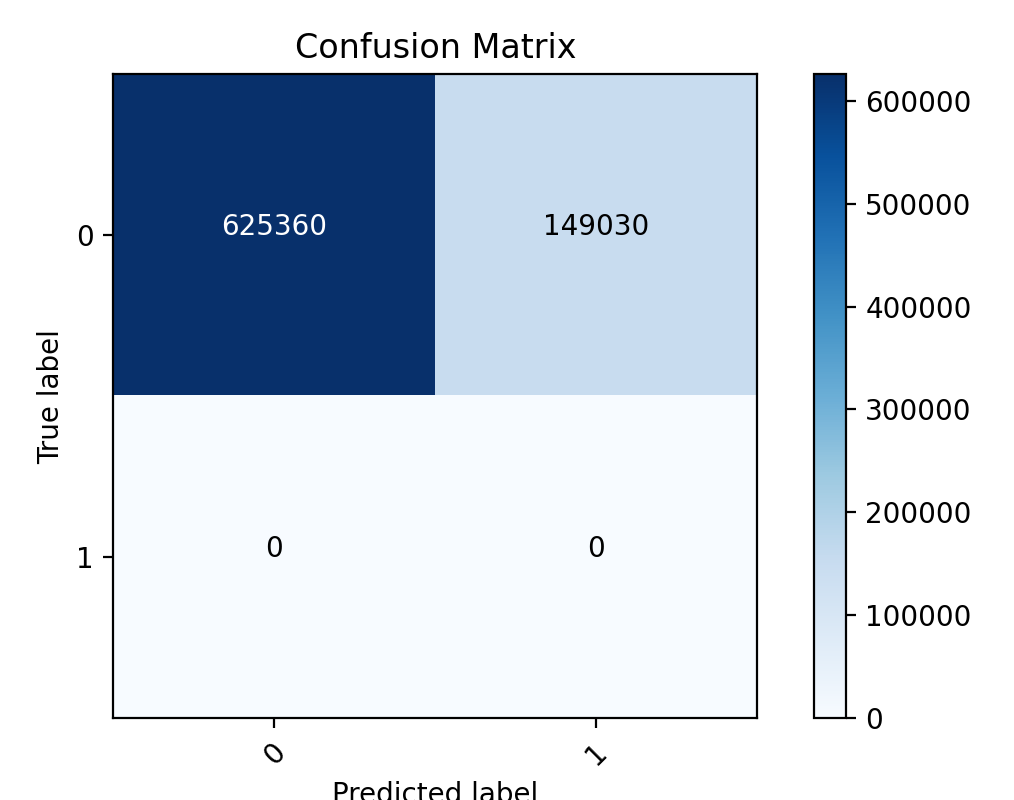
\includegraphics[width=\textwidth]{mlp-cm-no.png}
  \caption{Confusion Matrix for TS1.}
  \label{fig:mlp-cm-no}
\end{figure}

\subsection{Evaluation with TS2}
\label{sec:mlp-disc-ts2}
% low related hits:
% ROC AUC: 0.999
% ROC PR: 0.001
%%               precision    recall  f1-score   support

%%          0.0       1.00      0.91      0.96   5829395
%%          1.0       0.00      1.00      0.00        10

%%     accuracy                           0.91   5829405
%%    macro avg       0.50      0.96      0.48   5829405
%% weighted avg       1.00      0.91      0.96   5829405
%% F1: 0.0
%% F2: 0.0
\subsection{Evaluation with TS3}
\label{sec:mlp-disc-ts3}
%% medium related hits:
% ROC AUC: 0.978
% ROC PR: 0.009
%%               precision    recall  f1-score   support

%%          0.0       1.00      0.92      0.96   5879559
%%          1.0       0.00      0.98      0.00      1176

%%     accuracy                           0.92   5880735
%%    macro avg       0.50      0.95      0.48   5880735
%% weighted avg       1.00      0.92      0.96   5880735
%% F1: 0.005
%% F2: 0.011

\subsection{Evalution with TS4}
\label{sec:mlp-disc-ts4}
%% high related hits:
% ROC AUC: 0.959
% ROC PR: 0.334
%%               precision    recall  f1-score   support

%%          0.0       1.00      0.92      0.96    355859
%%          1.0       0.19      0.83      0.31      8372

%%     accuracy                           0.92    364231
%%    macro avg       0.59      0.87      0.63    364231
%% weighted avg       0.98      0.92      0.94    364231
%% F1: 0.311
%% F2: 0.497

% TODO discussion of results of best model

% ---------------------------------------------------------------------------
% ----------------------- end of thesis sub-document ------------------------
% ---------------------------------------------------------------------------
